% !TEX root=./whitepaper.tex
\section{Transactional Processing on Key-Value Store}

\project employs concurrency control in the key-value runtime to support transactional processing for concurrent operations on multiple keys. 
This concurrency control mechanism is optimistic and hinges on the total ordering of log entries enforced by the underlying log layer. 
Figure~\ref{fig:tx} illustrates the mechanism.

When an application server linking with the \project key-value runtime starts a transaction using \texttt{BeginTx()} interface, it notifies the runtime that the transaction will work on the current state snapshot constructed by playing the log to the current tail.
The further key-value operations before the invocation of \texttt{EndTx()} updates the key-values locally in the server without exposing the updates to the log. 
When \texttt{EndTx()} is invoked, the runtime composes a \emph{commit record} containing the log position the transaction starts from and the read-write set of the transaction.  
This commit record is then appended to the log.

\begin{figure}[H]	
	%\vspace{-6mm}
	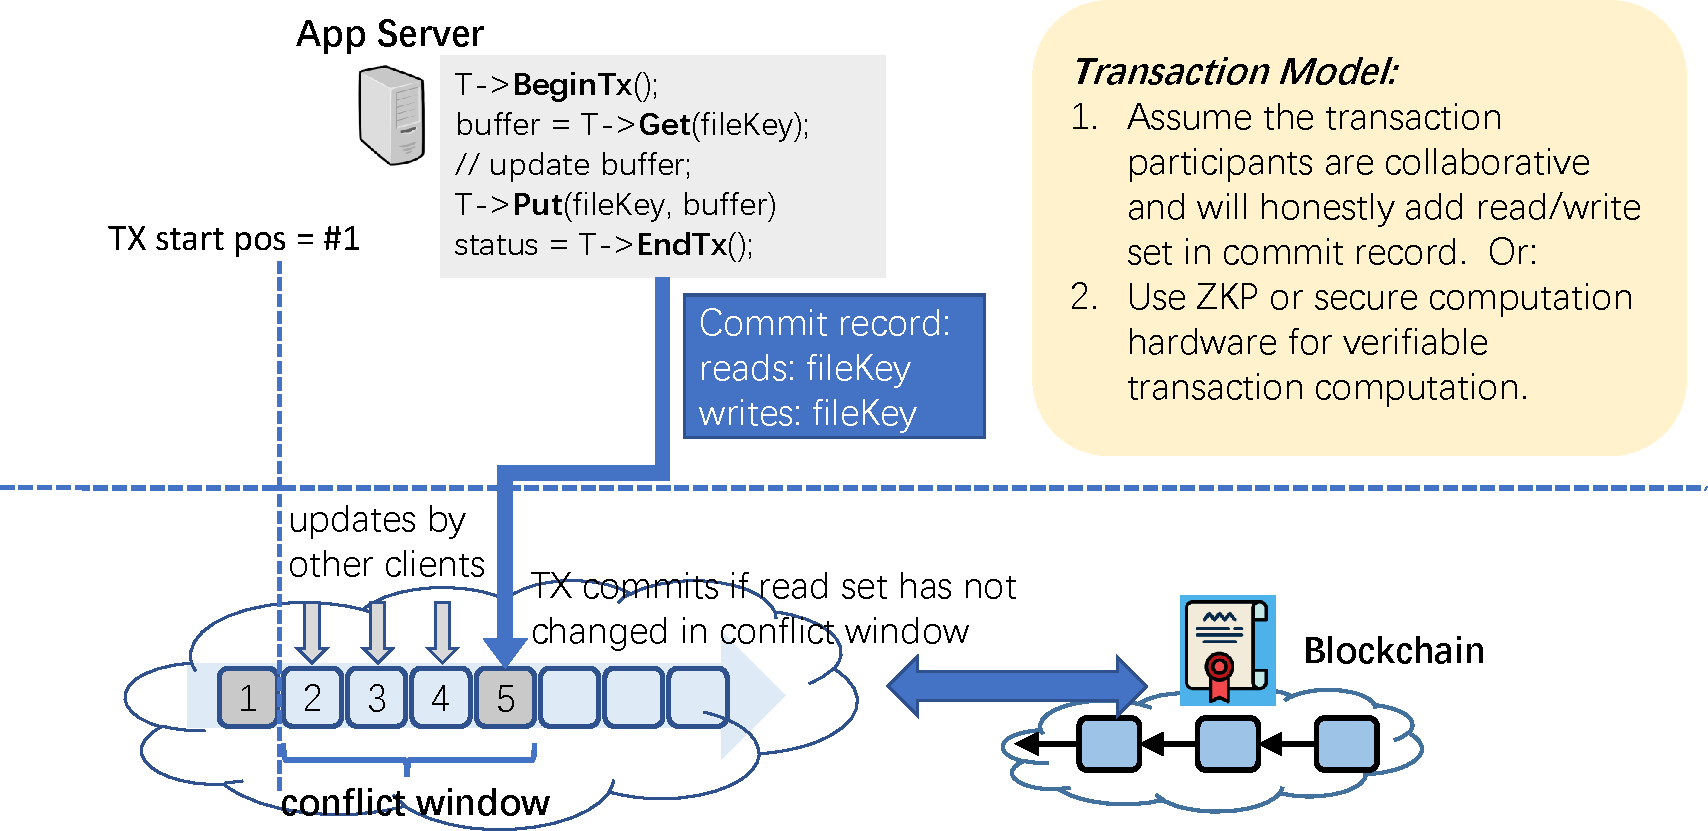
\includegraphics[width=\textwidth]{figure/tx-crop.pdf}
	\caption{Transactional Processing on \project KV Store}
	\label{fig:tx}
	%\vspace{-10mm}
\end{figure}
 
When an application server with the key-value runtime encounters the commit record during playing the log, it identifies a \emph{conflict window} consists of all the log entries between the start log position of the transaction and the position of the commit record. 
The log entries in the conflict window therefore contain the key-value operations concurrent with the transaction submitting the commit record. 
The runtime further detects whether these concurrent operations contain the updates on the keys that belong to the read set of the transaction.
If yes, the transaction is aborted, otherwise committed successfully.

This transaction model assumes that the transaction participants are collaborative and will honestly compose the commit record with correct content.
Although this assumption in decentralized environment is too strong, it is still achievable for specific applications. 
For example, for an application like Google Docs, a user normally shares the access to others who can be trusted. 
In case this assumption cannot hold, the code of the transaction can be stored in \project log and some mechanism of verifiable computation like zero-knowledge proof or hardware with trust execution environment (TEE) can be employed by the transaction executors to detect the validity of the commit record.

